\documentclass[10pt,a4paper,twoside]{article}
\usepackage[english]{babel}
\usepackage{amsmath}
\usepackage{braket}
\usepackage{amssymb,amsfonts,textcomp}
\usepackage{subfig}
\usepackage{graphicx}
\usepackage{float,flafter}
\usepackage{cite}
\usepackage{hyperref}
\usepackage[utf8]{inputenc}
\usepackage{float}
\usepackage{pgfplotstable,filecontents}
\setlength\paperwidth{20.999cm}\setlength\paperheight{29.699cm}\setlength\voffset{-1in}\setlength\hoffset{-1in}\setlength\topmargin{1.499cm}\setlength\headheight{12pt}\setlength\headsep{0cm}\setlength\footskip{1.131cm}\setlength\textheight{25cm}\setlength\oddsidemargin{2.499cm}\setlength\textwidth{15.999cm}
\newcommand{\apj}{The Astrophysical Journal}
\newcommand{\lambdabar}{{\mkern0.75mu\mathchar '26\mkern -9.75mu\lambda}}
\setcounter{section}{6}
\begin{document}
	\begin{center}
		\hrule
		\vspace{.4cm}
		{\bf {\huge Subatomic Physics II: Problem set 6}}
		\vspace{.2cm}
		\\
		{\bf Arthur Adriaens}
		\vspace{.2cm}
		\hrule
	\end{center}
\subsection{Helicity}
As parity violation is maximal in the V-\textit{minus}-A \textit{theory}, helicity defined as 
\begin{equation}
	h = \frac{\boldsymbol{s}\cdot\boldsymbol{p}}{|\boldsymbol{s}|\cdot|\boldsymbol{p}|}
\end{equation}
will change sign during a charged weak interaction, this is only possible if either $\boldsymbol{s}$ or $\boldsymbol{p}$ changes sign. We therefore have that if we consider the decay of a $\tau^+$ lepton with spin up this will preferably decay into a positron with spin up, antiparallel to the momentum. With the neutrino's traveling the other direction with positive helicity for the $\bar{\nu}_{\tau^+}$ and negative for the $\nu_{e^+}$ neutrino as (anti)neutrino's are always (right)left handed. For maximal positron momentum we thus have:
\begin{figure}[H]
	\centering
	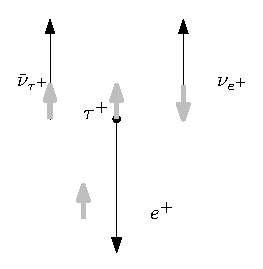
\includegraphics{decay.eps}
\end{figure}
\noindent
With the grey arrows representing the spins and the black arrows representing the momenta.
Considering the decay in the rest system we choose the electron to align with the x-axes:
\begin{figure}[H]
	\centering
	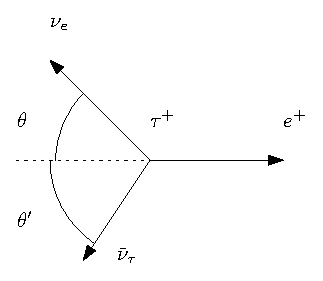
\includegraphics{interaction.eps}
\end{figure}
\noindent
We have the following four-vector equation:
\begin{equation}
	P_{\tau^+} = P_{e^+} + P_{\nu_e} + P_{\bar{\nu}_{\tau}}
\end{equation}
And thus
\begin{equation}
P_{\tau^+} - P_{\bar{\nu}_{\tau}}= P_{e^+} + P_{\nu_e}
\end{equation}
which we can square to:
\begin{equation}
	m_{\tau}^2 - 2m_{\tau}|\boldsymbol{p_{\bar{\nu}_{\tau}}}| = m_{e^+}^2+2\left(E_{e^+}|\boldsymbol{p_{\nu_{e}}}| - |\boldsymbol{p_{\nu_{e}}}|\cdot|\boldsymbol{p_{e^+}}|\cos(\theta)\right)
\end{equation}
And thus the energy of the positron has a spectrum following
\begin{equation}
	E_{e^+} = \frac{m_{\tau}^2 - 2m_{\tau}|\boldsymbol{p_{\bar{\nu}_{\tau}}}| - m_{e^+}^2}{2|\boldsymbol{p_{\nu_{e}}}|} + |\boldsymbol{p_{e^+}}|\cos(\theta)
\end{equation}
Which is maximal if $\theta = 0$ implying the neutrino's traveling parallel (conservation of three-momentum) directly away from the positron as we expect.
\subsection{Particle hunting using the Dalitz plot}
\subsubsection*{Bevatron}
The unit in the plot is in squared BeV which stands for $10^9$ elektronvolts, equivalent to today's GeV. The name comes from the Bevatron particle accelerator at Lawrence Berkeley National Laboratory, U.S., which began operating in 1954\cite{Lawrence}. This was a proton synchrotron which accelerated protons into a fixed target with energies up to billions of electronvots (from which the name of the accelerator, \textbf{B}illions of \textbf{eV} Synchro\textbf{tron}, came and thus the unit).
\subsubsection*{Electric charge, I(J$^P$) and strangeness}
Mostly from appendix C of "Modern particle physics"\cite{Thomson}:
\begin{center}
	\begin{tabular}{c|c|c|c}
		Hadron & Q(e) & I(J$^P)$ & S\\
		\hline
		p & +1 & $\frac{1}{2}(\frac{1}{2}^+)$ & 0\\
		$\pi^+$ & +1 & 1($0^-$)& 0\\
		K$^-$ & -1 & $\frac{1}{2}(0^-)$ & -1\\
		$\pi^-$ & -1 & 1($0^-$) & 0\\
		$\Lambda$ & 0 & 0($\frac{1}{2}^+$) & -1\\
	\end{tabular} 
\end{center}
\subsubsection*{Number of intermediate resonances}
From the plot we can read off 2 resonances, $X_1$ at a $\Lambda\pi^-$ pair mass of $\approx$1380MeV with the $\Lambda\pi^+$ pair mass ranging between $\approx$1500 and 1700MeV and $X_2$ at a $\Lambda\pi^+$ pair mass of $\approx$1380MeV with the $\Lambda\pi^-$ pair mass between $\approx$1500 and 1700MeV. $X_1$ decays into $\Lambda\pi^-$ and $X_2$ decays into $\Lambda\pi^+$:
\begin{figure}[H]
	\centering
	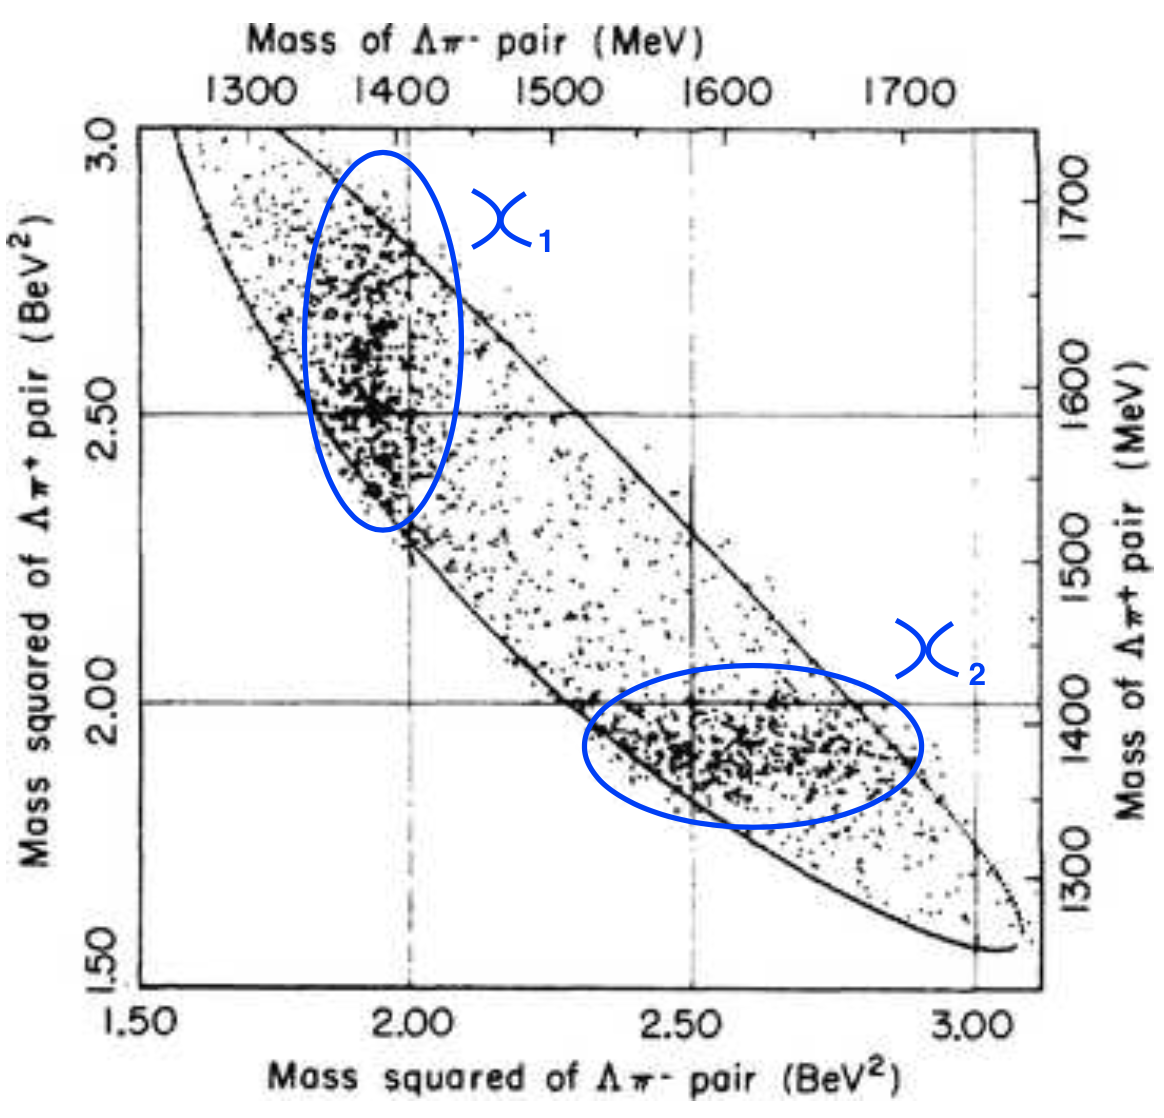
\includegraphics[width=0.5\textwidth]{resonanties.png}
\end{figure}
\subsubsection*{Mesons, baryons or anti-baryons?}
For this we can take a look at the strictly conserved baryon number of the involved particles, the initial state has $B_{tot} = 1$ (also from appendix C, knowing that mesons have B=0 and baryons B=1). As the intermediate state has $\pi^{\pm}$ with B=0, the resonances $X_i$ have to be baryons. 
\subsubsection*{Electric charges and strangeness quantum numbers}
As charge and strangeness are conserved quantities in the strong interaction we can just look at the difference in these numbers for the final and initial particles:\\\\
For $pK^-\rightarrow X_1\pi^+$ on the left hand side we have $Q_{tot}=0$ and $S_{tot} = -1$, as $\pi^+$ has S=0 and a charge of 1 this means that $X_1$ must have a charge of -1 and a strangeness of -1.
\\\\
For $pK^-\rightarrow X_2\pi^-$ on the left hand side we have $Q_{tot}=0$ and $S_{tot} = -1$, as $\pi^-$ has S=0 and a charge of -1 this means that $X_2$ must have a charge of 1 and a strangeness of -1.
\subsubsection*{masses}
The masses of the $X_i$-baryons must be around $\approx$1380MeV as this is the mass of the $\Lambda\pi^{\pm}$ pair at which the resonances occur.
\subsubsection*{Strong isospin I and I$_z$}
As the resonances decay into $\Lambda\pi^{\pm}$ we can couple their isospin ($\ket{0,0}\otimes\ket{1,\pm1}$),  to arrive at $\ket{1,\pm1}$. $X_1$ thus has $\ket{I,I_z} = \ket{1,-1}$ and $X_2$ has $\ket{I,I_z} = \ket{1,1}$.
\subsubsection*{possibilities for J$^P$ restricting \textit{l} to 0 or 1}
As $X_i$ decays into particles $\pi^{\pm}$ and $\Lambda$ with J$^P$ respectively 0$^-$ and $\frac{1}{2}^+$, the expected J$^P$ of the $X_i$ baryons is either $\frac{1}{2}^-$ (if $\Delta$\textit{l} =0) or $\frac{3}{2}^+$ (if $\Delta$\textit{l} =1 $\implies$ $P = (-1)\times(1)\times(-1)^\textit{l} = 1$).
\subsubsection*{identify X$_i$ if J=3/2}
The Resonances are $\Sigma^*$ (sigma) baryons as they have a mass of 1385MeV $\approx 1380$MeV. Their main decay modes are $\Lambda\pi$ and $\Sigma\pi$. In particular, looking at the charges, we can see that $X_1$ corresponds to $\Sigma(1385)^-$ with decay modes $\Lambda\pi^-$ and $\Sigma^0\pi^-$ and $X_2$ to $\Sigma(1385)^+$ with decay modes $\Lambda\pi^+$ and $\Sigma^0\pi^+$
\bibliography{sources}
\bibliographystyle{plain}
\end{document}
